\chapter{Introduction}
\label{chpt:introduction}

% explain the core SAC signaling cascade vs RZZ pathway

% Unlike the kinetochore-localized signaling activity of tightly clustered \protein{Knl1} molecules, the eSAC is a diffusible, cytosolic complex of two proteins.  

\begin{figure}
    \centering
    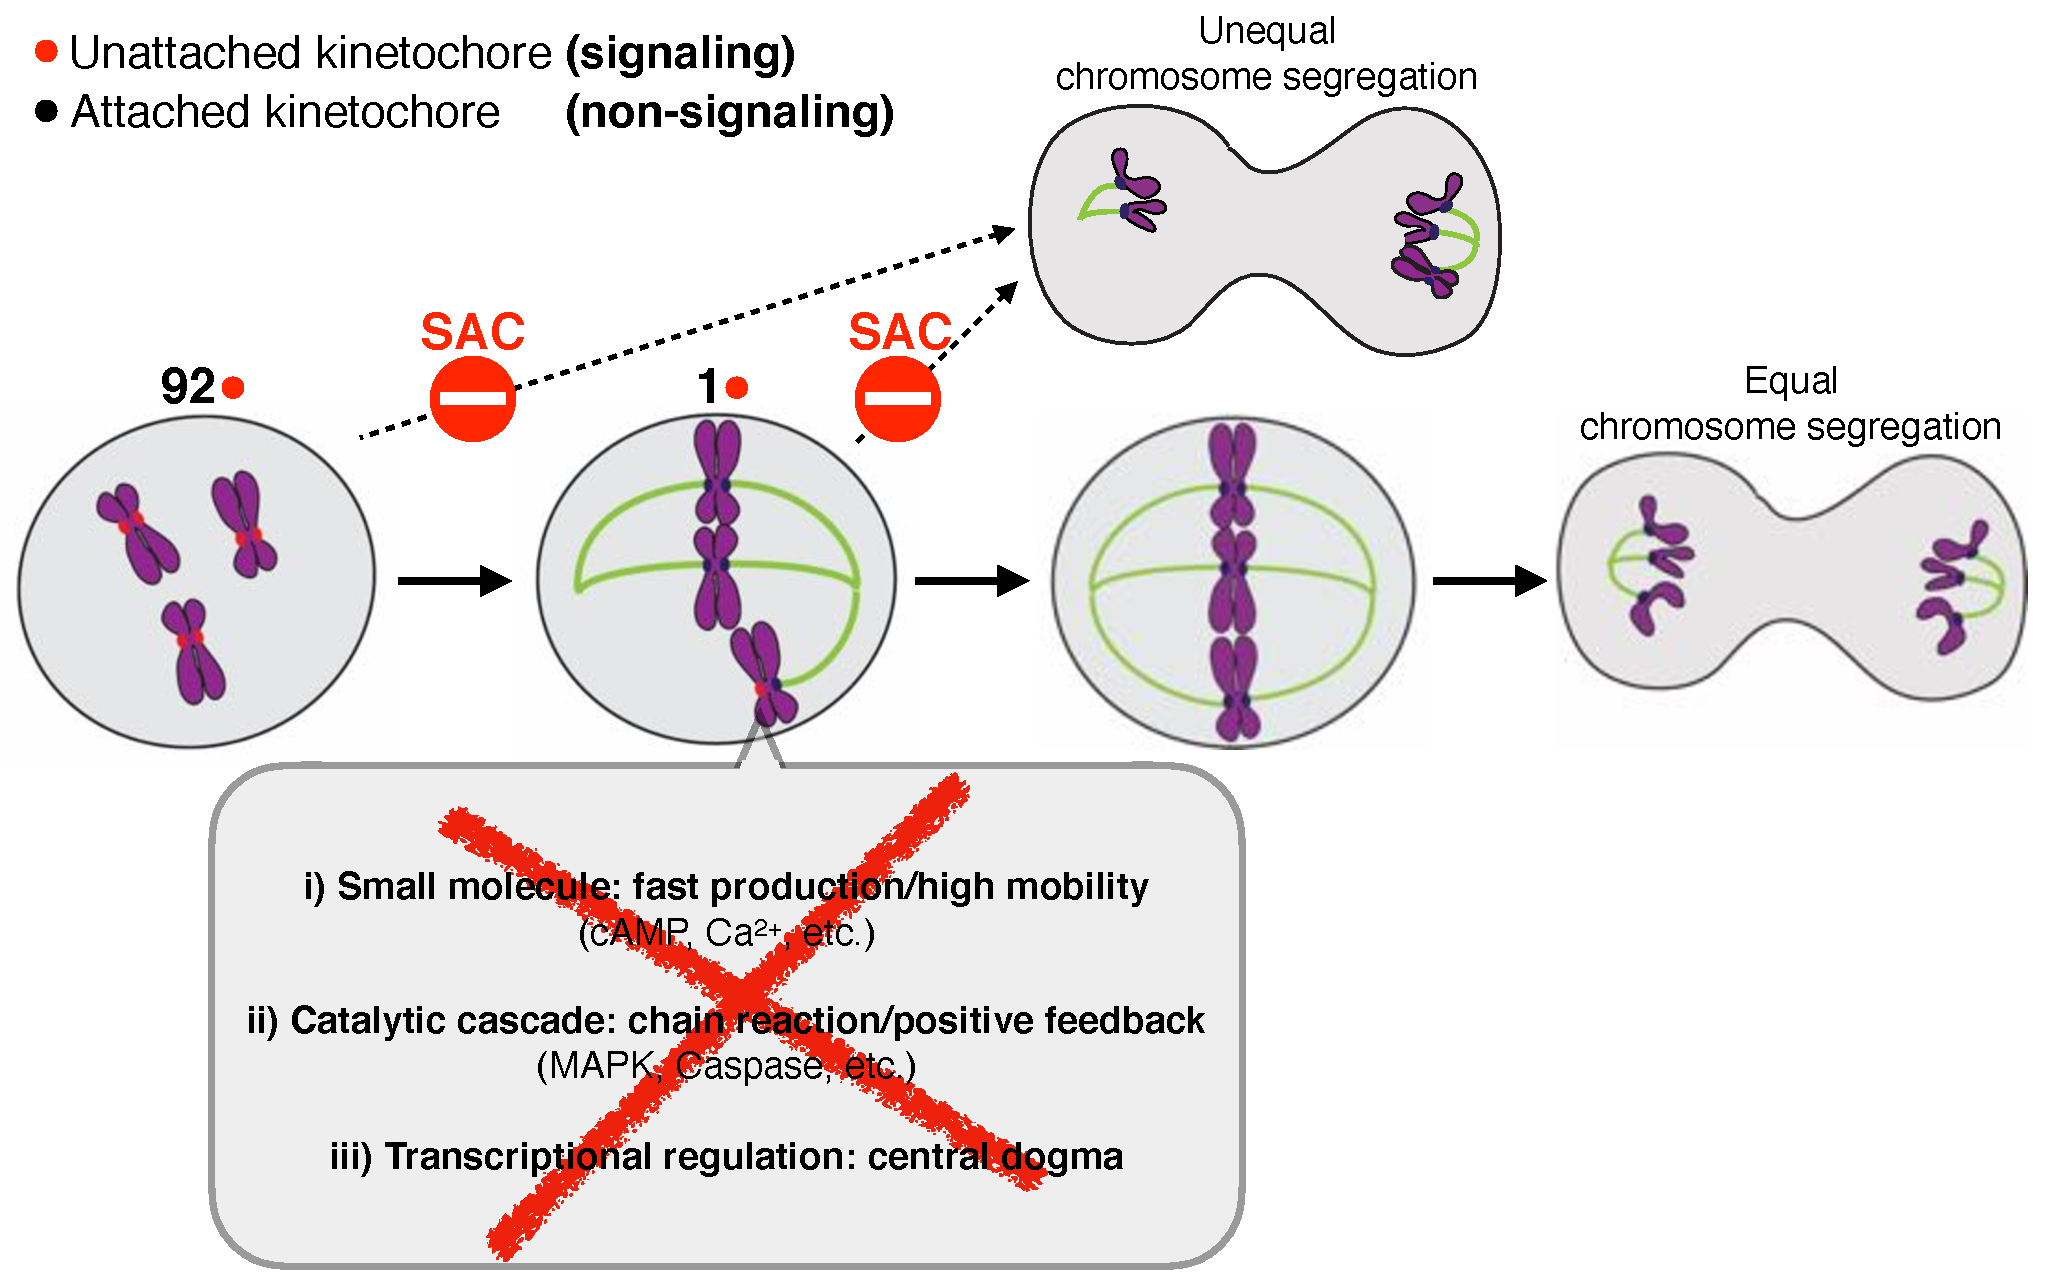
\includegraphics[width=0.95\textwidth]{chapters/figures/Introduction.pdf}
    \caption{\textbf{A diagram illustrating the role and properties of the spindle assembly checkpoint (SAC).}}
    \label{Introduction}
\end{figure}